% --------------------------------------
% Document Class
% --------------------------------------
\documentclass[a4paper,11pt]{article}
% --------------------------------------



% --------------------------------------
% Use Package
% --------------------------------------


\usepackage[francais]{babel}
\usepackage{ucs}
\usepackage[utf8]{inputenc}
\usepackage[T1]{fontenc}

\usepackage{makeidx}
\usepackage{color}
\usepackage{graphicx}
\usepackage{float}
\usepackage[hidelinks]{hyperref} 
\usepackage{geometry}
%\usepackage{lastpage}
%\usepackage{marginnote}
\usepackage{fancyhdr}
%\usepackage{titlesec}
%\usepackage{framed}
\usepackage{amsmath}
\usepackage{empheq}
\usepackage{array}
\usepackage{multicol}
\usepackage{csquotes}
%\usepackage{adjustbox}

% insert code
\usepackage{listings}

% define our color
\usepackage{xcolor}

% code color
\definecolor{ligthyellow}{RGB}{250,247,220}
\definecolor{darkblue}{RGB}{5,10,85}
\definecolor{ligthblue}{RGB}{1,147,128}
\definecolor{darkgreen}{RGB}{8,120,51}
\definecolor{darkred}{RGB}{160,0,0}

% other color
\definecolor{ivi}{RGB}{141,107,185}

\def\verticaltext#1{\rotatebox[origin=c]{90}{\x{#1}}}


\lstset{
    language=python,
    captionpos=b,
    extendedchars=true,
    frame=lines,
    numbers=left,
    numberstyle=\tiny,
    numbersep=5pt,
    keepspaces=true,
    breaklines=true,
    showspaces=false,
    showstringspaces=false,
    breakatwhitespace=false,
    stepnumber=1,
    showtabs=false,
    tabsize=3,
    basicstyle=\small\ttfamily,
    backgroundcolor=\color{ligthyellow},
    keywordstyle=\color{ligthblue},
    morekeywords={include, printf, uchar},
    identifierstyle=\color{darkblue},
    commentstyle=\color{darkgreen},
    stringstyle=\color{darkred},
}


% --------------------------------------



% --------------------------------------
% Page setting
% --------------------------------------
%\pagestyle{empty}
\setlength{\headheight}{15pt}

\setcounter{secnumdepth}{3}
\setcounter{tocdepth}{2}

\makeatletter
\@addtoreset{chapter}{part}
\makeatother 

\hypersetup{       % parametrage des hyperliens
  colorlinks=true,  % colorise les liens
  breaklinks=true,  % permet les retours à la ligne pour les liens 
                    % trop longs
  urlcolor= blue,   % couleur des hyperliens
  linkcolor= black, % couleur des liens internes aux documents 
                    % (index, figures, tableaux, equations,...)
  citecolor= green  % couleur des liens vers les references 
                    % bibliographiques
}

% --------------------------------------

% --------------------------------------
% Information
% --------------------------------------
\title{
  \noindent\hrulefill \\
  \vspace{10mm} Compte-rendu ICP : Iterative Closest Point
}

\author{Gaëtan DEFLANDRE}
% --------------------------------------

\definecolor{myColor}{rgb}{0.5, 0.1, 0.75}

% --------------------------------------
% Begin content
% --------------------------------------
\begin{document}


\maketitle

\noindent\hrulefill \\


\section{Introduction}

L'imagerie 3D et l'analyse des formes 3D sont des domaines de recherche 
de pointe. Nous retrouvons les résultats de ces recherches dans 
l'imagerie médicale, les outils de modélisations 3D et maintenant dans 
les interactions temps réel.\\

Dans ce compte rendu, nous allons voir l'un des principes de base en 
analyse de forme 3D, l'algorithme ICP\footnote{Iterative Closest Point}. 
Cet algorithme permet de retrouver la meilleure correspondance entre 
deux modèles 3D.\\

\newpage

\section{Principe d'ICP}

Lorsque nous disposons de deux modèles 3D qui se ressemblent, il est 
intéressant de retrouver la meilleure correspondance entre ces deux 
modèles. Nous utilisons donc ICP\cite{121791}, qui recherche une 
translation et une rotation qui minimise l'erreur entre les points 
des deux modèles.\\

\subsection{Avant-propos et nommage}

Soit:
\begin{itemize}
  \item les données d'un nuage de points $D$, en entrée, qui sublir les
  transformations.
  \item un autre nuage de points $M$, le modèle de référence en entrée.
  \item la translation 3D $t$ et la rotation 3D $R$.
  \item l'erreur $E(R,t)$ entre le nuage de points $M$ et $D$ transformé 
  avec $R$ et $t$.
  \item $SVD$\footnote{singular value decomposition} est la 
  décomposition en valeurs singulières.\\
\end{itemize}

Le terme générique ``forme'' correspond au nuage de point 3D de l'un des 
modèles d'entrée.\\

\subsection{Problématique}

Nous recherchons la translation $t$ et rotation $R$ à appliquer à la 
forme $D$. Cette transformation $(R,t)$ doit minimiser l'erreur $E$ 
entre la forme $D$ et $M$.

$$
min(dist(R*D+t,M))
$$
\\

\subsection{Fonctionnement d'ICP}

L'algorithme ICP consiste en plusieurs itérations qui vont converger 
vers une erreur $E$ minimal. Afin de retrouver la transformation $(R,t)$ 
optimale.\\

\subsubsection{Algorithme}

Entrées:
\begin{itemize}
  \item La forme $M$.
  \item La forme $D$.
  \item Les conditions d'arrêt des itérations (nombre d'itérations 
  \ldots).\\
\end{itemize}

\begin{description}
  \item[$\bullet$]Itérer
  \begin{description}
     \item[-] Faire une table de correspondance entre les points de $D$ 
     et les points de $M$.
     \item[-] Calculer la transformation $(R,t)$ qui minimise l'erreur, 
     c'est-à-dire, la distance entre les points correspondants.
     \item[-] Appliquer la transformation trouvée à la forme $D$.\\
   \end{description} 
\end{description}

\subsubsection{Table de correspondance}

Pour chaque point $D_i$ de $D$, nous cherchons le plus proche point 
dans la forme $M$. Pour cela, nous calculons la distance euclidienne 
entre $D_i$ et les points de $M$. Nous conservons dans une table de 
correspondance des plus proches points, les paires de points qui ont une 
distance euclidienne minimale.\\

La table de correspondance a donc une taille de $|D|$.\\

\subsubsection{Transformation minimisant l'erreur}

La meilleure transformation pour une itération (pour la table de  
correspondance calculé à cette itération), minimise l'erreur de 
distance entre les points correspondants.\\

Il existe plus fonction permettant de calculer cette erreur de 
distance $E(R,t)$:
\begin{itemize}
  \item point-to-point
  \item point-to-plane
  \item scaled\\
\end{itemize}

\paragraph{Théorème de convergence}
L'algorithme d'ICP converge toujours vers une distance locale minimale 
avec une fonction erreur respectant la moyenne des carrés.\\

Nous détaillons, ici, la fonction erreur ``point-to-point'' décrite en 
cours.

\begin{equation}
  E(R,t)=\sum\limits_i^{|D|} ||(R*D_i+t)-M_i||^2
\end{equation}

$M_i$ est le point correspondant au point $D_i$ dans la table de 
correspondance.\\

\begin{align}
  min(E(R))&=\sum\limits_i^{|D|} ||R*D'_i+R*\bar{D_i}+t+\bar{t}-M'_i||^2 \\
  min(E(R))&=\sum\limits_i^{|D|} ||R*D'_i-M'_i||^2
\end{align}
car,
\begin{align}
  R*\bar{D}+t &= \bar{t} \\
  t &= \bar{t} - R*\bar{D}
\end{align}

De plus, nous avons la propriété suivante:
\begin{equation}
  ||a-b||^2=(a-b)^t.(a-b)
\end{equation}
\\

Donc, $R=uv^t$ avec $SVD(\frac{1}{|D|}\sum D_i^tM_i) = u\sum v^t$

\begin{figure}[H]
  \begin{center}
    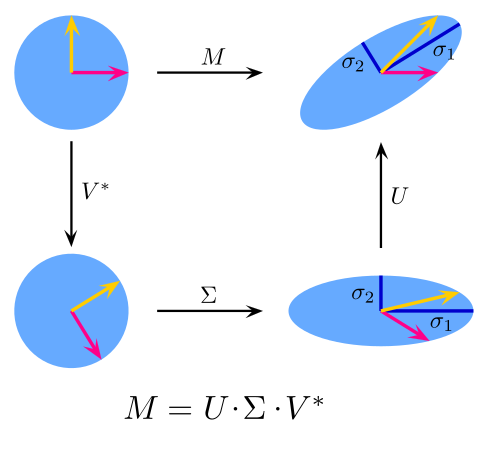
\includegraphics[width=200px]{SingularValueDecomposition.png}
    \caption{Décomposition en valeurs singulières}
  \end{center}
\end{figure}

Si $(R,t)$ est la transformation optimale alors $D$ et $M$ ont un centre 
masse identique.\\

\newpage

\section{Conclusion}

L'algorithme d'ICP est capable de retrouver la meilleure correspondance 
entre deux formes 3D en entrée. Seul la position des points de ces 
formes 3D est utile.\\

ICP est algorithme robuste au bruit et efficace. Il fonctionne avec 
tout type de modèles en entrés et il est couramment utilisé en temps 
réel. Il existe des améliorations de cet algorithme, mais ICP reste 
très utilisé en imagerie 3D.\\

\bibliographystyle{ieeetr}
\bibliography{biblio}

\end{document}
